\documentclass{article}
\usepackage[utf8]{inputenc}
\usepackage{amssymb}
\usepackage{amsmath}
\usepackage{graphicx}
\graphicspath{{Images/}}

\setlength{\oddsidemargin}{0in}
\setlength{\textwidth}{6.5in}
\setlength{\topmargin}{-.55in}
\setlength{\textheight}{9in}
\pagestyle{empty}


\title{Scientific Computation HW1}
\author{Michael Nameika}

\begin{document}


\maketitle

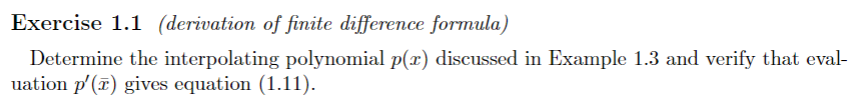
\includegraphics[scale = 0.8]{ex1.1.PNG}

Since we are given three points $x_0 = \bar{x} - 2h$, $x_1 = \bar{x} - h$, and $x_2 = \bar{x}$, the quadratic interpolant for $x_0, x_1, x_2$, $p(x)$ will be unique. That is, we may use any interpolating polynomial we like. I will be using a Lagrange interpolating polynomial. Recall that a quadratic Lagrange interpolating polynomial is given by

\[p(x) = y_0\frac{(x-x_1)(x-x_2)}{(x_0 - x_1)(x_0 - x_2)} + y_1\frac{(x - x_0)(x - x_2)}{(x_1 - x_0)(x_1 - x_2)} + y_2\frac{(x - x_0)(x - x_1)}{(x_2 - x_0)(x_2 - x_1)}\]

where $y_0, y_1, y_2$ are the values we wish to interpolate and $x_0, x_1, x_2$ are the associated $x$ values. 

Using this formula, we find the following interpolating polynomial:

\[p(x) = u(\bar{x} - 2h)\frac{(x - (\bar{x} - h))(x - \bar{x})}{((\bar{x} - 2h) - (\bar{x} - h))((\bar{x} - 2h) - \bar{x})} + u(\bar{x} - h)\frac{(x - (\bar{x} - 2h))(x - \bar{x})}{((\bar{x} - h) - (\bar{x} - 2h))((\bar{x} - h) - \bar{x})} + \dotsb\]
\[\dotsb + u(\bar{x})\frac{(x - (\bar{x} - 2h))(x - (\bar{x}-h))}{((\bar{x} - (\bar{x} - 2h))(\bar{x} - (\bar{x} - h))}\]

Simplifying and expanding, we find

\[p(x) = u(\bar{x} - 2h)\frac{x^2 - (\bar{x} - h)x - x\bar{x} + \bar{x}(\bar{x} - h)}{2h^2} - u(\bar{x} - h)\frac{x^2 - x(\bar{x} - 2h) - \bar{x}x + \bar{x}(\bar{x} - 2h)}{h^2} + \dotsb\]
\[\dotsb + u(\bar{x})\frac{x^2 - x(\bar{x}-2h) - \bar{x}x + \bar{x}(\bar{x} - 2h)}{2h^2}\]

Now, we need to find the derivative of $p(x)$ and evaluate at $x = \bar{x}$. Differentiating the $p(x)$ above and simplifying, we find

\[p'(x) = u(\bar{x} - 2h)\frac{2x + h - 2\bar{x}}{2h^2}  - u(\bar{x} - h)\frac{2x +2h - 2\bar{x}}{h^2} + u(\bar{x})\frac{2x + 3h - 2\bar{x}}{2h^2}\]

Plugging in $x = \bar{x}$ into the above equation for $p'(x)$, we find
\[p'(\bar{x}) = \frac{1}{2h}(u(\bar{x} - 2h) - 4u(\bar{x} - h) + 3u(\bar{x}))\]
Which is what we wished to show.
\newline\newline

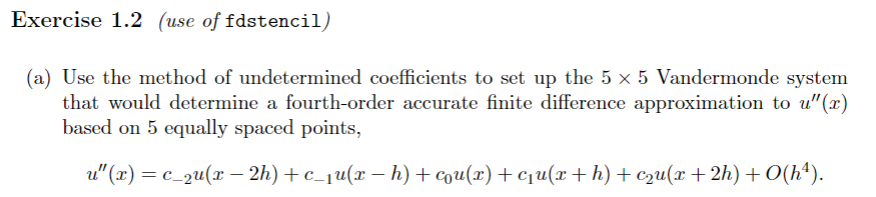
\includegraphics[scale = 0.8]{ex1.2a.PNG}
\newline

We wish to set up a $5 \times 5$ Vandermonde matrix to determine a fourth order accurate centered difference approximation for $u''(x)$ with $5$ equally spaced points, $x_0 = \bar{x} - 2h$, $x_1 = \bar{x} - h$, $x_2 = \bar{x}$, $x_3 = \bar{x} + h$, $x_4 = \bar{x} + 2h$. To begin, let's expand $u(x)$ around the above $5$ points:

\[u(\bar{x} - 2h) = u(\bar{x}) - 2hu'(\bar{x}) + \frac{(2h)^2}{2}u''(\bar{x}) - \frac{(2h)^3}{3!}u'''(\bar{x}) + \frac{h^4}{4!}u''''(\bar{x})  + \mathcal{O}(h^5)\]

\[u(\bar{x} - h) = u(\bar{x}) -hu'(\bar{x}) + \frac{h^2}{2!}u''(\bar{x}) - \frac{h^3}{3!}u'''(\bar{x}) + \frac{h^4}{4!}u''''(\bar{x}) + \mathcal{O}(h^5)\]

\[u(\bar{x}) = u(\bar{x})\]

\[u(\bar{x} + h) = u(\bar{x}) + hu'(\bar{x}) + \frac{h^2}{2!}u''(\bar{x}) + \frac{h^3}{3!}u'''(\bar{x}) + \frac{h^4}{4!}u''''(\bar{x}) + \mathcal{O}(h^5)\]

\[u(\bar{x} + 2h) = u(\bar{x}) + 2hu'(\bar{x}) + \frac{(2h)^2}{2!}u''(\bar{x}) + \frac{(2h)^3}{3!}u'''(\bar{x}) + \frac{(2h)^4}{4!}u''''(\bar{x}) + \mathcal{O}(h^5)\]

Multiplying the above equations by $c_{-2}$, $c_{-1}$, $c_0$, $c_1$, $c_2$ respectively, and summing them up, we find the following five equations to solve for the second derivative

\[c_{-2} + c_{-1} + c_0 + c_1 + c_2 = 0\]

\[-2hc_{-2} - hc_{-1} + hc_1 + 2hc_2 = 0\]

\[\frac{(2h)^2}{2!}c_{-2} + \frac{h^2}{2!}c_{-1} + \frac{h^2}{2!}c_1 + \frac{(2h)^2}{2!}c_2 = 1\]

\[-\frac{(2h)^3}{3!}c_{-2} - \frac{h^3}{3!}c_{-1} + \frac{h^3}{3!}c_1 + \frac{(2h)^3}{3!}c_2 = 0\]

\[\frac{(2h)^4}{4!}c_{-2} + \frac{h^4}{4!}c_{-1} + \frac{h^4}{4!}c_1 + \frac{(2h)^4}{4!} = 0\]

Writing as a matrix system, we get 
\[
\begin{bmatrix}
    1 & 1 & 1 & 1 & 1\\
    -2h & -h & 0 & h & 2h\\
    \frac{(2h)^2}{2!} & \frac{h^2}{2!} & 0 & \frac{h^2}{2!} & \frac{(2h)^2}{2!}\\
    -\frac{(2h)^3}{3!} & -\frac{h^3}{3!} & 0 & \frac{h^3}{3!} & \frac{(2h)^3}{3!}\\
    \frac{(2h)^4}{4!} & \frac{h^4}{4!} & 0 & \frac{h^4}{4!} & \frac{(2h)^4}{4!}\\

\end{bmatrix}
\begin{bmatrix}
    c_{-2}\\
    c_{-1}\\
    c_{0}\\
    c_1\\
    c_2\\
\end{bmatrix}
 = 
 \begin{bmatrix}
    0\\
    0\\
    1\\
    0\\
    0\\
 \end{bmatrix}
\]

Plugging the system into MATLAB and solving, we find

\[
\begin{bmatrix}
    c_{-2}\\
    c_{-1}\\
    c_0\\
    c_1\\
    c_2\\
\end{bmatrix}
=
\begin{bmatrix}
    -\frac{1}{12h^2}\\
    \frac{4}{3h^2}\\
    -\frac{5}{2h^2}\\
    \frac{4}{3h^2}\\
    -\frac{1}{12h^2}\\
\end{bmatrix}
\]

We wish to show that these coefficients give an $\mathcal{O}(h^4)$ approximation. From the Taylor expansion at the beginning of the problem, we expanded to $\mathcal{O}(h^5)$ and since the coefficients have a $\frac{1}{h^2}$ term, this suggests that our method is $\mathcal{O}(h^3)$. However, including the fifth order terms for the Taylor expansion gives us the following equation:
\[-\frac{1}{12h^2}\frac{(-2h)^5}{5!} + \frac{4}{3h^2}\frac{(-h)^5}{5!} + \frac{4}{3h^2}\frac{h^5}{5!} - \frac{1}{12h^2}\frac{(2h)^5}{5!}\]
\[ = 0\]
So our method will return an $\mathcal{O}(h^4)$ approximation.

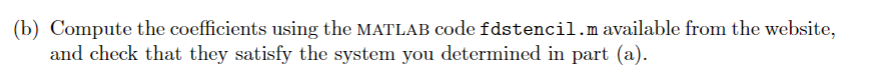
\includegraphics[scale = 0.8]{ex1.2b.PNG}
\newline

Using the fdstencil.m script, we find the following coefficients

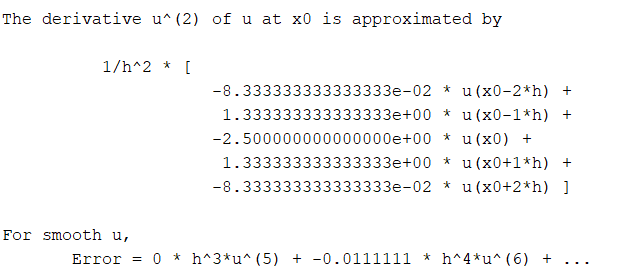
\includegraphics[]{fdstencilcoeff.PNG}
\newline
Which are exactly the coefficients given by the Vandermonde system in part a).
\newline

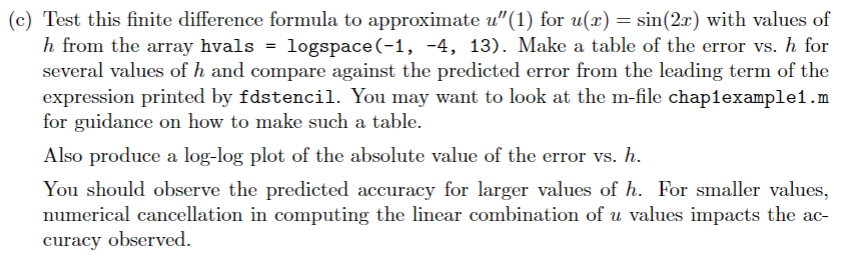
\includegraphics[scale = 0.8]{ex1.2c.PNG}
\newline

For this problem, denote the approximation for the second derivative by $D_2(x)$. Using the stencilScript.m code I wrote (see attached m file), we find the following table for error versus $h$ values:

\begin{center}
    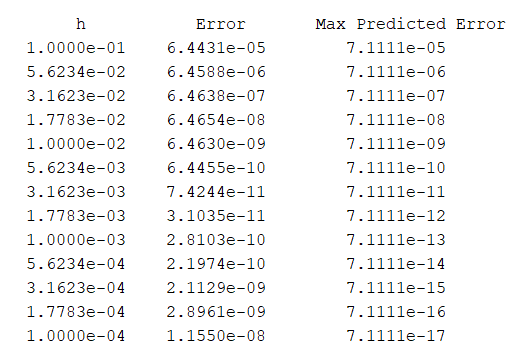
\includegraphics[scale = 0.8]{err and pred err2.PNG}
\end{center}

Notice that the maximum predicted error has the same order of magnitude of the measured error until the value of $h$ drops below approximately $3.16 \times 10^{-3}$.
\newline

We also find the following loglog plot for the error:

\begin{center}
    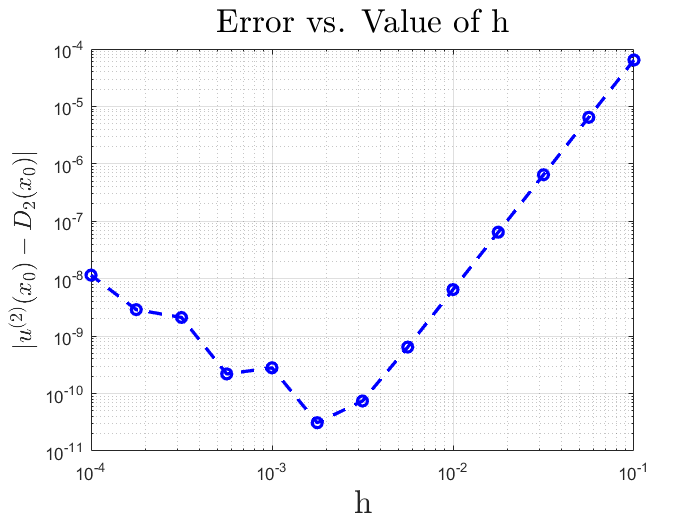
\includegraphics[scale = 0.6]{error_vs_h_plot.png}
\end{center}

We notice from the above plot that numerical error begins to take over when $h < 3.16 \times 10^{-3}$, as mentioned above.

\end{document}
